\section{Chemical Consistency}\label{sec:const}
There are three primary areas in which must the stellar models must be made chemically
consistent: the atmospheric boundary conditions, the opacities, and interior
abundances. The interior abundances are relatively easily handled by adjusting
parameters within our stellar evolutionary code. However, the other two areas are
more complicated to bring into consistency. Atmospheric boundary conditions and
opacities must both be calculated with a consistent set of chemical abundances
outside of the stellar evolution code. For evolution we use the Dartmouth Stellar Evolution Program (DSEP) \citep{Dotter2008}, a well tested 1D stellar evolution code which has a particular focus on modelling low mass stars ($\le 2$ M$_{\odot}$)

\subsection{Atmospheric Boundary Conditions}\label{sec:atm}
Certain assumptions, primarily that the radiation field is at equilibirum and radiative transport is diffusive \citep{Salaris2005}, made in stellar structure
codes, such as DSEP, are valid when the optical depth of a star is small.
However, in the atmospheres of stars, the number density of particles drops low
enough and the optical depth consequently becomes large enough that these
assumptions break down, and separate, more physically motivated, plasma modeling code is required.
Generally structure code will use tabulated atmospheric boundary conditions
generated by these specialized codes ATLAS9 \citep{Kurucz1993}, PHEONIX \citep{Husser2013}, MARCS \citep{Gustafsson2008}, and MPS-ATLAS \citep{Kostogryz2023}. Often, as the boundary conditions are both expensive to compute
and not the speciality of stellar structure researchers, the boundary
conditions are not updated as as light-element interior abundance varies. 

One key element when chemically consistently modeling NGC 2808 modeling is the
incorporation of new atmospheric models with the same elemental abundances as
the structure code. We use atmospheres generated from the \texttt{MARCS} grid of
model atmospheres \citep{Plez2008}. \texttt{MARCS} provides one-dimensional,
hydrostatic, plane-parallel and spherical LTE atmospheric models
\citep{Gustafsson2008}. Model atmospheres are made to match the
spectroscopically measured elemental abundances of populations A and E.
Moreover, for each populations, atmospheres with  various helium mass fractions
are generated. These range from Y=0.24 to Y=0.36 in steps of 0.02. A comparison
of the pressure and temperature throughout the atmospheres of the two
populations with helium abundances representative of literature values is shown
in Figure \ref{fig:AEAtmComp}.

\begin{figure}
	\centering
	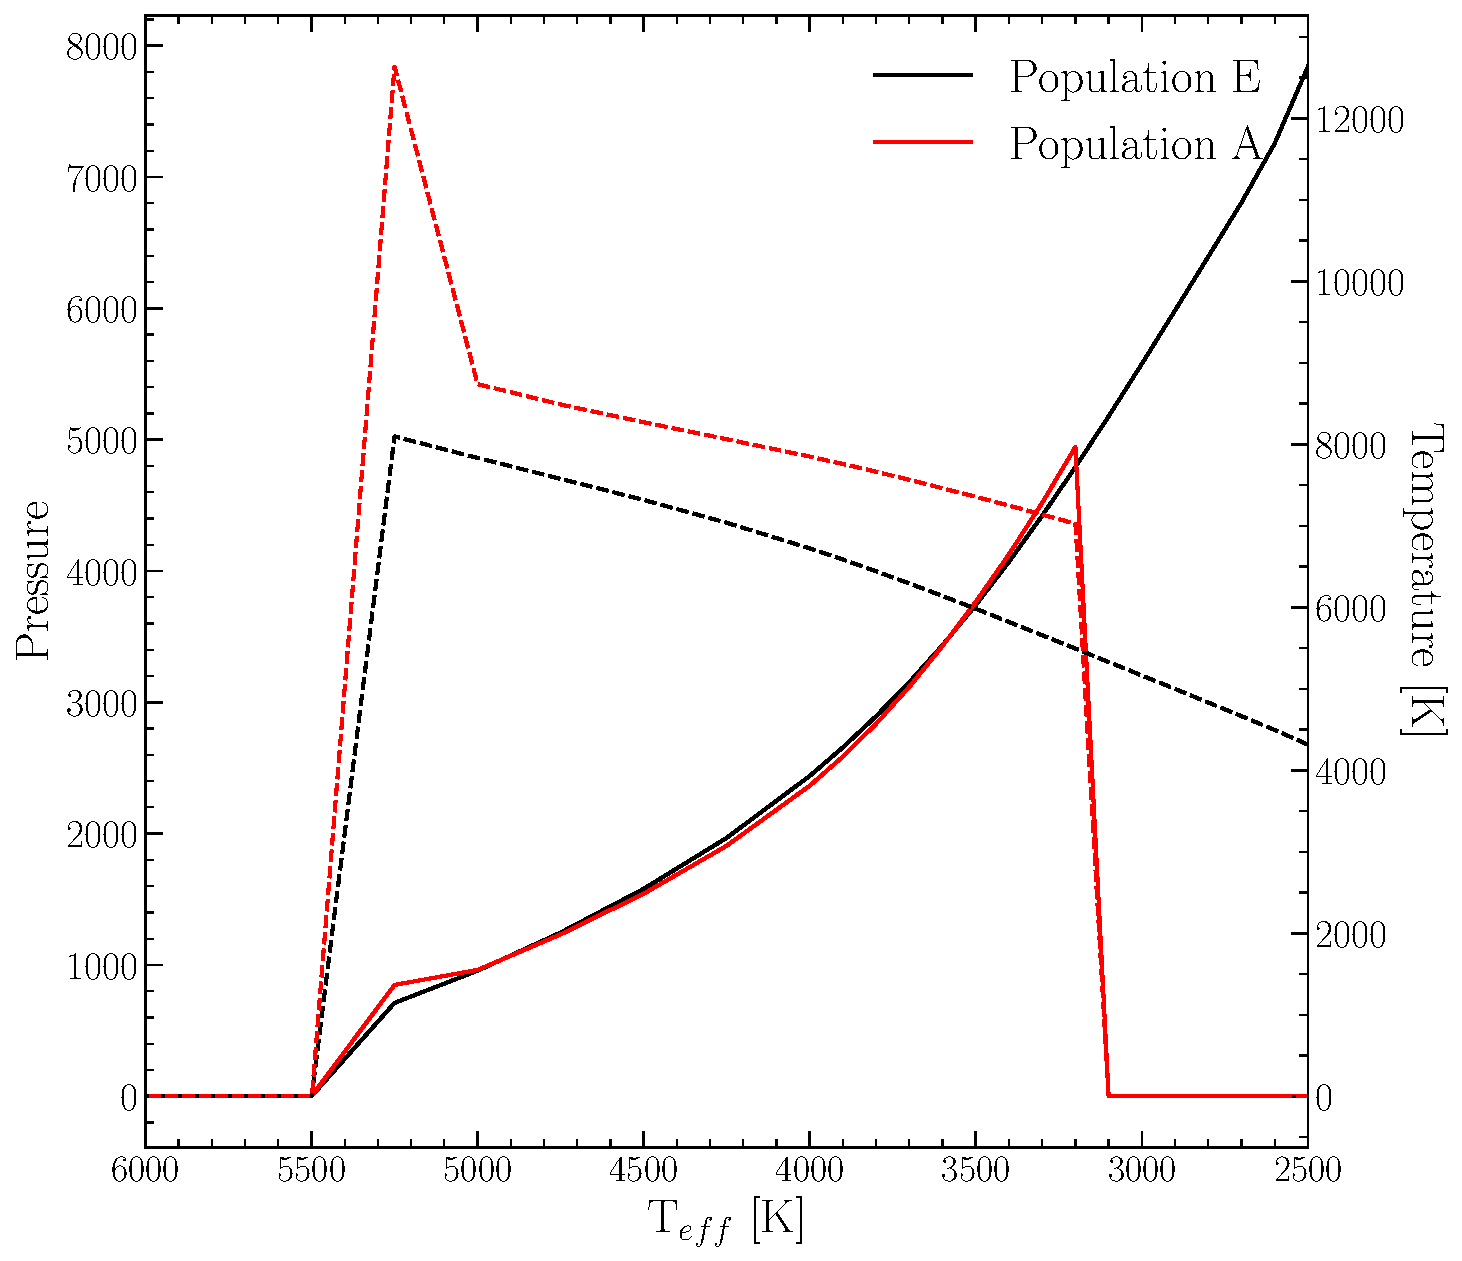
\includegraphics[width=0.5\textwidth]{src/figures/notebookFigures/AtmosphereComparison.pdf}
	\label{fig:AEAtmComp}
	\caption{Comparison of the MARCS model atmospheres generated for the two
	extreme populations of NGC 2808. These lines shows population A and E with
	the same Helium abundance; though, we fit a grid of models over various
	helumn abundances. Dashed lines show the temperature of the boundary
	condition while sold lines show the pressure.}
\end{figure}


\subsection{Opacities}\label{sec:opac}
In addition to the atmospheric boundary conditions, both the high and low
temperature opacities used by DSEP must be made chemically consistent. Here we
use OPLIB high temperature opacity tables \citep{Colgan2016} retrieved using
the TOPS web-interface. Low temperature opacity tables are retrieved from the
Aesopus 2.0 web-interface \citep{Marigo2009, Marigo2022}. Ideally, these
opacities would be the same used in the atmospheric models. However, the
opacities used in the MARCS models are not publicly available. As such, we use
the opacities provided by the TOPS and Aesopus 2.0 web-interfaces.
